% vim:ft=tex:
%
\documentclass[12pt]{article}
\usepackage[margin=1in]{geometry}
\usepackage{graphicx}

\begin{document}

\pagenumbering{gobble}

\begin{center}
  \textbf{Interaction Techniques and Active Learning Methods for Mixed Initiative Exploration of Fabrication Hardware Parameter Spaces}\\
  \vspace{.5em}
  Andrew Head
\end{center}

As you enter the Invention Lab---Berkeley's student hackerspace---you'll see evidence that getting started with fabrication hardware is hard.
Scorched cardboard sits the scrap pile from laser cutting jobs that caught on fire.
Dozens of failed 3D prints line the foyer walls from thin supports or severe overhangs.
% As you walk into the foyer of Berkeley's student hackerspace, you see dozens of failed 3D prints lined up along the walls.
% These tell a solemn truth:
% Getting started with fabrication hardware is hard.
% 3D printing without large enough tolerances leaves movable parts stationary.
% Thin supports or sharp overhangs result in tangled spindles of ABS that fail to layer properly.
%When using a laser cutter, vector cutting with the power set too high lights the workpiece on fire.
This work seeks to \textbf{improve the efficiency and effectiveness of early, exploratory interactions with fabrication machines.}

I will focus improving the user experience of of rastering images onto arbitrary materials using a laser cutter.
Rastering is the process of ``etching'' an image into a work piece with with a dot matrix of laser fixations.
Four parameters---power, speed, frequency, and resolution---control the depth, speed, and fidelity of the image is rastered (Figure~\ref{fig:rasters}).
Many values for these parameters can cause the material to scorch.

The proposed research aims for a vision for fabrication machines that will be able to assist users in helping them to learn their parameters, models of operation, and constraints.
I propose that a laser cutter that follows active learning can help a user more efficiently explore the space of possible parameters and converge on an optimal set of parameters.

% for a new material, or to systematically vary these parameters until a raster.
% The values of these are vary based on the material a user is working with, the speed they want to work to get done with, the depth of the marks, and how rough of a sketch they can accept for the current raster.
% A major failure occurs in that the hacker will likely want to use the machine long before they want to develop an accurate mental model of how the parameters impact the work to be done.

% There is no clear way how learning from demonstration techniques can be used to describe configurations for settings such as laser power, speed, frequency, and resolution.
% Furthermore, these parameters don't map directly to the task the user wants to perform.
% The hacker may have a clear idea of the appearance of the material surface that they want to attain, and an understanding of how these parameters cause it just is not clear.

This work aims to answer the following questions that, to my knowledge, are open questions within both the fields of human-robot interaction and the fabrication concentration of human-computer interaction.
First, \textbf{how can a robot learn an ideal configuration for a task when no demonstration is given?}
Second, \textbf{what are the most efficient subjective inputs and interaction techniques to enable fast convergence to an ideal configuration with a fabrication machine?}

This study will begin with an observational study with student members of the Invention Lab (around $n=5$).
These students will be interviewed to better understand the frequency, severity, and types of errors students encounter expressing designs to fabrication hardware.
Questions will include:
What jobs have you submitted in the past that have failed?
How many times did you have to iterate on this artifact before it was successfully fabricated?
What did you learn about the capabilities of the hardware after this effort?

Then I will implement an active learning scheme~\cite{settles_active_2010} that will collect user ratings for raster jobs based on example configurations of power, speed, resolution and frequency for a laser cutter, with the aim of predicting user ratings with a minimum number of examples.
While active learning in typical contexts (see~\cite{settles_active_2010}) has been applied to learning linear decision boundaries for binary classification, we will draw upon past work that seeks to adapt active learning to predicting continuous values for examples (e.g.~\cite{sugiyama_active_2008}).
Currently, I suspect that a Gaussian kernel function or a quadratic curve will best express a user's perception of the quality of a configuration in actualizing their design.

I will conduct a study to determine what input methods will be most successful in helping a user converge to a desired rastering configuration.
The usability study will be run in the Invention Lab with the Universal Laser Systems VLS3.50 machine, for which I have already received clearance to run user studies.
Subjects will be provided with a work piece they are asked to replicate.
One experimenter will direct the VLS3.50 to perform one raster job with configuration examples derived from the algorithm described above remotely (so that it is opaque to the participant).
The participant will be asked to rate each example, providing a score that will be fed back into the active learning algorithm.
After every third example, the model show the participant a raster with the optimal score according to the model learned so far.
The raster will be considered `complete' if the user offers it the top score on the Likert scale.
Subjects will all be exposed to three input methods via a simple web interface that connects back to the active learner:
Likert-scale ratings of the most recent example, arrangement of rank of all seen examples so far, and trial and error (no active learning, but manual configuration of parameters only.)

Given the limits of the hardware available in the Invention Lab, this study will likely include around 4 testers altogether.
Measurements collected will include the time and iterations taken to perform the task, Likert scale ratings of user satisfaction, and qualitative feedback about strategies to achieve the ideal rastering.

\begin{figure}
  \centering
  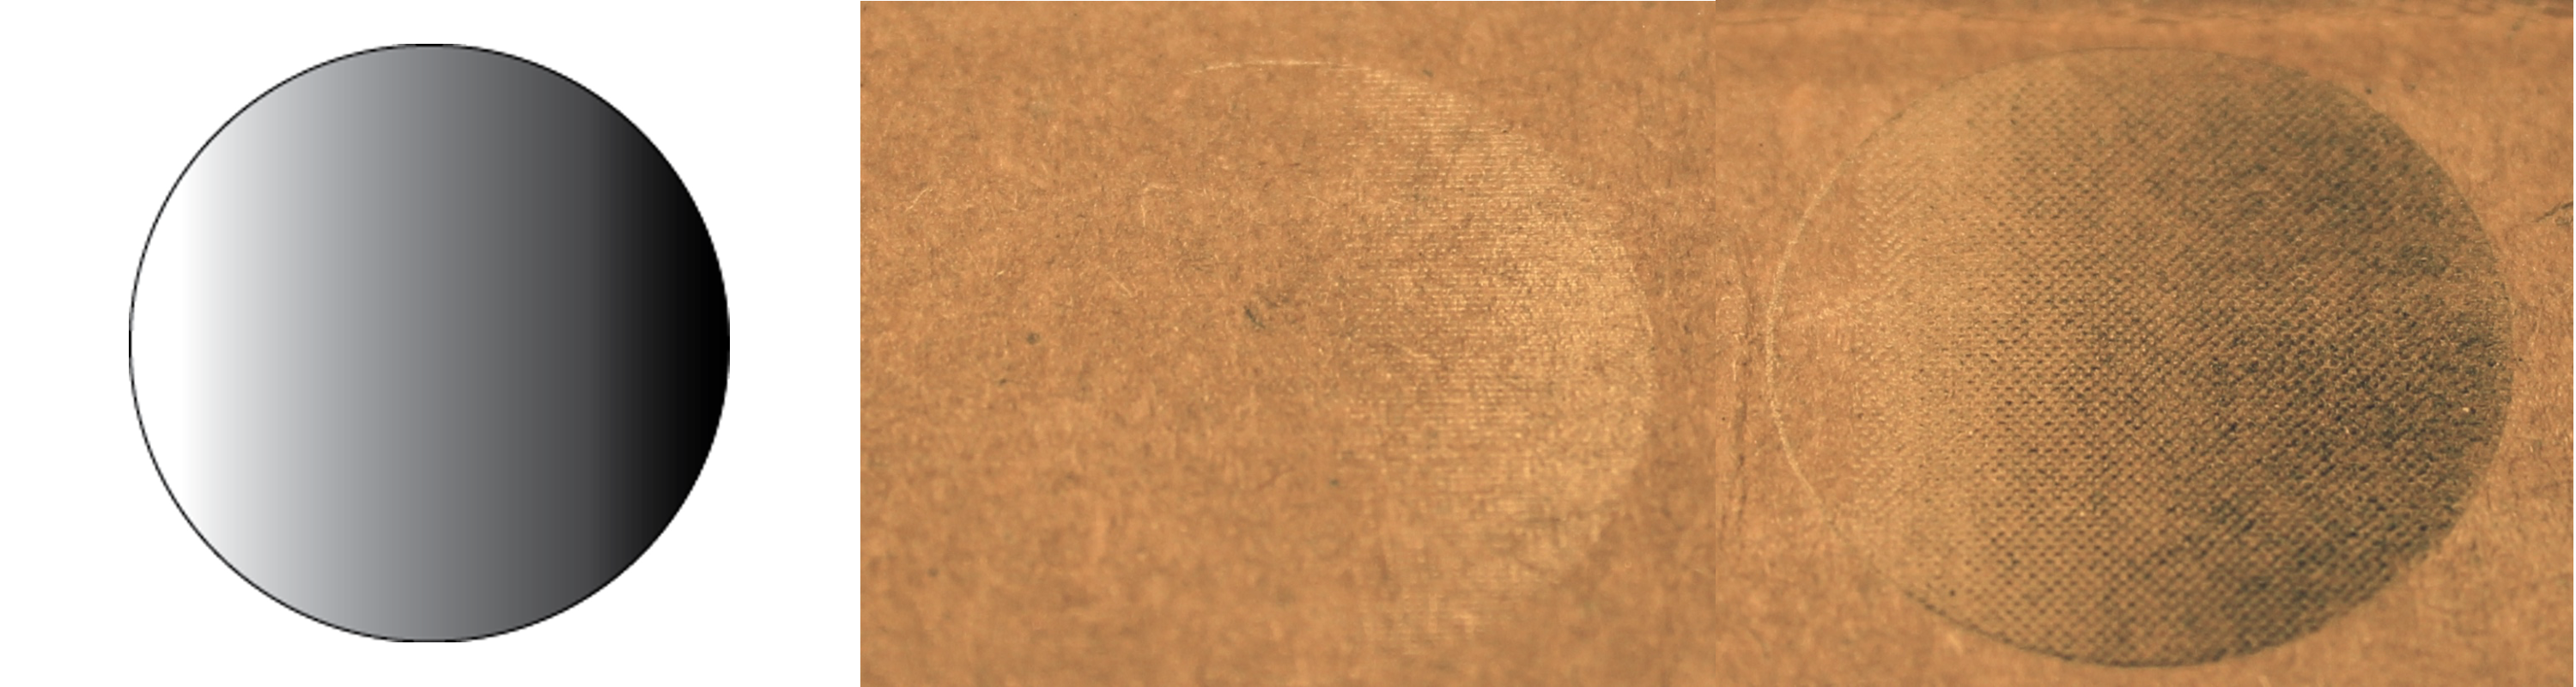
\includegraphics[width=0.6\textwidth]{figures/rasters}
  \caption{\small{%
  A drawing `rastered' into cardboard by a laser cutter with two different configurations.
  \emph{Left}: the original image given to the laser cutter.
  \emph{Center}: an etching that is too faint to see due to low power
  \emph{Right}: an etching that scorched the cardboard due to high power and low speed.
  A user of the laser cutter will have to manipulate the laser's parameters to get the desired appearance.}}
\label{fig:rasters}
\end{figure}

\end{document}
